\section{Objectives of this study}
As shown by equation \ref{eq:reflection_chiral}, the chiral medium acts as a reflector for circularly right polarised light\footnote{This is true for a right-handed medium. A left-handed medium would act as a reflector for circularly right polarised light.}. This hints three geometries to try to improve the purity of the outputted mode. 

The first idea is to introduce a defect in a chiral cavity. Thus, it is hoped that modes of the handedness of the medium would be able to exist within the defect, while being confined by the distributed mirrors on each side. This geometry is shown in figure \ref{fig:defect}.

The second idea is to simulate a hybrid cavity, consisting of a right-handed medium providing gain between two left-handed media without gain. This geometry is presented in figure \ref{fig:hybrid}. Thus, only left-circularly polarised light would be able to bounce on the reflectors and right-circularly polarised light would not be allowed in the gain medium.

The third idea consist in using a combination of the two first ideas, \textit{i.e.} a hybrid cavity where a defect has been introduced at the centre. This geometry is shown in figure \ref{fig:hybrid_defect}.

After reproducing the past results obtained in a simple cavity (shown in figure \ref{fig:simple_cavity}), the three other cavities will be studied to determine their ability to produce circularly polarised light when pumped.

\begin{figure}
	\centering
	\begin{subfigure}{0.40\linewidth}
		\includegraphics[width=\linewidth]{images/simple_cavity}
		\caption[Simple cavity]{Simple cavity}
		\label{fig:simple_cavity}
	\end{subfigure}
	\begin{subfigure}{0.58\linewidth}
		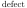
\includegraphics[width=\linewidth]{images/defect.png}
		\caption{Cavity with a defect}
		\label{fig:defect}
	\end{subfigure}
	\begin{subfigure}{\linewidth}
		\includegraphics[width=\linewidth]{images/hybrid.png}
		\caption{Hybrid cavity}
		\label{fig:hybrid}
	\end{subfigure}
	\begin{subfigure}{\linewidth}
		\includegraphics[width=\linewidth]{images/hybrid_defect.png}
		\caption{Hybrid defect cavity}
		\label{fig:hybrid_defect}
	\end{subfigure}
	\caption[Cavities modelled in this study]{Cavities modelled in this study.  For every cavity, $\bar{n}$ denotes an average refractive index, $\delta n$ a birefringence and $p=\frac{2\pi}{L_p}$ a periodicity. They are surrounded by isotropic media of refractive indices $n_1$ and $n_2$. The cavity lengths are an integer multiple of $L_p$.}
	\label{fig:cavities_blender}
\end{figure}